\chapter{Scientific Programming}
\label{ch:SciProg}

The introduction of the computer around World War II had a major impact on the mathematical fields of science. Previously unsolvable problems were now solvable. The question was no longer whether or not it was possible, but rather to what precision and with which method. The computer spawned a new branch of physics, \textit{computational physics}, redefining the limits of our understanding of nature. The first major result of this synergy between science and computers came with the infamous atomic bombs \textit{Little Boy} and \textit{Fat Man}, a product of \textit{The Manhattan Project} lead by \textit{J. Robert Oppenheimer} \cite{supermen}. 

\section{Programming Languages}

Programming is the art of writing computer programs. A program is a list of instructions for the computer, commonly referred to as \textit{code}. It is in many ways similar to human-to-human instructions; for instance, different programming languages may be used to write instructions, such as \textit{C++}, \textit{Python} or \textit{Java}, as long as the recipient is able to translate it. The instructions may be translated prior to the execution, i.e~the code is \textit{compiled}, or it may be translated \textit{run-time} by an \textit{interpreter}. 

The native language of the computer is \textit{binary}: Ones and zeros, which corresponds to high - and low voltage readings. Every character, number, color, etc. is on the lowest level represented by a sequence of binary numbers referred to as \textit{bits}. In other words, programming languages serve as a bridge between the binary language of computers and a more manageable language for everyday programmers.

The closer the programming language at hand is to pure processor (CPU) instructions\footnote{The CPU is the part of the computer responsible for flipping bits.}, the lower the \textit{level} of the language is. This section will introduce high- and low level languages, focusing on C++ and Python, as these are the most commonly used languages throughout this thesis.   


\subsection{High-level Languages}

Scientific programming involves a vast amount of different tasks, all from pure visualization and organization of data, to efficient memory allocation and processing. For less CPU-intensive tasks, the runtime of the program is so small that the efficiency becomes irrelevant, leaving languages which prefer simplicity and structure over efficiency the optimal tool for the job. These languages are referred to as \textit{high-level languages} \footnote{There are different definitions of the distinction between high- and low-level languages. Languages such as \textit{assembly} is extremely complex and close to machine code, leaving all machine-independent languages as high-level in comparison. However, for the purpose of this thesis, the distinction will be set at a higher level than assembly.}.

High-level codes are often short snippets designed with a specific aim such as analyzing raw data, administrating input and output from different tools, creating a \textit{Graphical User Interface} (GUI), or \textit{gluing} different programs, which are meant to be run sequentially or in parallel, together into one. These short specific codes are referred to as \textit{scripts}, hence high-level languages designed for these tasks are commonly referred to as \textit{scripting languages}\cite{inf3331, pythonBook}. 

Some examples of high-level languages are Python, Ruby, Perl, Visual Basic and UNIX shells. Excellent introductions to these languages are found throughout the World Wide Web.

\subsubsection{Python}
\label{sec:Python}

Named after the infamous \textit{Monte Python's flying circus}, Python is an easy to learn open source interpreted programming language invented by Guido van Rossum around 1990. Python is designed for optimized development time by having a very clean and rigorous coding syntax \cite{inf1100, pythonBook}. 

To demonstrate the simplicity of Python, consider the following simple expression

\begin{equation}
 S = \sum_{i=1}^{100} i = 5050.  \label{eq:sum100},
\end{equation}

which is calculated in Python by the following expression:

\lstinputlisting[language=Python]{../CodeInputs/Sum100Python.py}

Executing the script yields the expected result:

\begin{verbatim}
~$ python Sum100Python.py 
5050
\end{verbatim}

For details regarding the basics of Python, see Ref. \cite{inf1100}, or Ref. \cite{inf3331} for more advanced topics.  


\subsection{Low-level Languages}
\label{sec:lowlevel}

Scientific programming often involves solving complex equations. Complexity does not necessarily imply that the equations themselves are hard to understand; frankly, this is often not the case. In most cases of for example linear algebra, the problem at hand can be boiled down to solving $\mathbf{A}\mathbf{x} = \mathbf{b}$, however, the complexity lies in the dimensionality of the problem at hand. Matrix dimensions often range as high as millions. With each element being a double precision number (8 bytes or 64 bits), it is crucial to have full control of the memory and execute operations as efficiently as possible. 

This is where lower level languages excel. Hiding few to none of the details, the power is in the hand of the programmer. This, however, comes at a price: More technical concepts such as memory pointers, declarations, compiling, linking, etc. makes the development process slower than that of a higher-level language. 

Moreover, requesting access to an uninitialized element outside the bounds of an allocated array, Python will provide a detailed error message with proper traceback, whereas the compiled C++ code would simply crash runtime, leaving nothing but a ``segmentation fault'' for the user. The payoff comes when the optimized program ends up running for days, in contrast to the high-level implementation which might end up running for months.

In addition, several options to optimize compiled machine code are available by having the compiler rearrange the way instructions are sent to the processor. Details regarding memory latency optimization will be discussed in Section \ref{sec:CPUcache}. 

\subsubsection{C++}

C++ is a programming language developed by Bjarne Stroustrup in 1983. It serves as an extension to the original \textit{C} language, adding \textit{object oriented} features, that is, classes etc. \cite{ORegan}. The following code is a C++ implementation of the sum in Eq.~\ref{eq:sum100}:

\vspace{0.5 cm}
\lstinputlisting[language=c++]{../CodeInputs/Sum100C++.cpp}

\begin{verbatim}
~$ g++ Sum100C++.cpp -o sum100C++.x
~$ ./sum100C++.x 
5050
\end{verbatim}


Notice that, unlike Python, C++ requests an explicit declaration of \textit{S} as an integer variable. This in turn tells the compiler the exact amount of memory needed to store the variable, opening up the possibility of efficient memory optimization. 

Even though this is an extremely simply example, it illustrates the difference in coding styles between high- and low-level languages. The next section will cover the basics needed to understand object orientation in C++, and how it can be used to develop generalized coding frameworks.

\section{Object Orientation}
\label{sec:OO}

The concept of classes and objects were introduced for the first time in the language \textit{Simula 67}, developed by the Norwegian scientists Ole-Johan Dahl and Kristen Nygaard at the Norwegian Computing Research Center \cite{ORegan}. Object orientation quickly became the state-of-the-art in programming, and has ever since enjoyed great success in numerous computational fields. 

Object orientation ties everyday intuition into the programming language. Humans are object oriented without noticing it, in the sense that the focus is around \textit{objects} of \textit{classes}, for instance, an animal of a certain species, artifacts of a certain culture, people of a certain country, etc. This fact renders object oriented codes extremely readable compared to what is possible with standard functions and variables. In addition to simple object structures, which in some sense can be achieved with standard C \textit{structs}, classes provide functionality such as \textit{inheritance} and accessibility control. These concepts will be the focus for the rest of the chapter, however, for the sake of completeness, a brief introductory to class syntax is given.

\subsection{A Brief Introduction to Essential Concepts}

\subsubsection{Members}

A class in its simplest representation is a collection of variables and functions unique to a specified object of the class\footnote{Members can be shared by all class instances in C++ by using the static keyword. This will make the variables and function obtainable without initializing an object as well.}. When an object is created, it is uniquely identified by its own set of member variables.

An important member of a class is the object itself. In Python, this intrinsic mirror image is called \verb+self+, and must, due to the interpreter nature of the language, be present in all function calls. In C++, it is available in any class member function as the \verb+this+ pointer. Making changes to \verb+self+ or \verb+this+ inside a function is equivalent to changing the object outside the function. It is nothing but a way for an object to have access to itself at any time.

\subsubsection{Constructors}

The constructor is the class function responsible for initializing new objects. When requesting a new instance of a class, a constructor is called with specific input parameters. In Python, the constructor is called \verb+__init__()+, while in C++, the name of the constructor must match that of the class, e.g. \verb+someClass::someClass()+\footnote{The double colon notation means ``someClass' member someClass()''.}.

Creating a new object is simply done by calling the constructor

\begin{lstlisting}
someClass* someObject = new SomeClass("constructor argument");
\end{lstlisting}

The constructor can then assign values to member variables based on the input parameters.

\subsubsection{Destructors}

Opposite to constructors, destructors are responsible for deleting an object. In Python this is automatically done by the \textit{garbage collector}, however, in C++ this is sometimes important in order to avoid memory leaks. The destructor is implemented as the function \verb+someClass::~someClass()+, and is invoked by typing e.g. \verb+delete someObject;+.

Reference \cite{inf1100} is suggested for further introduction to basic concepts of classes.  

\subsection{Inheritance}

Consider the abstract idea of a keyboard: A board and keys (obviously). In object orientation terms, the keyboard \textit{superclass} describes a board with keys. It is \textit{abstract} in the sense that no specific information regarding the formation or functionality of the keys is needed in order to define the concept of a keyboard.

On the other hand, there exist different specific kinds of keyboards, e.g. computer keyboards or musical keyboards. Although quite different in design and function, they both relate to the same concept of a keyboard described previously: They are both \textit{subclasses} of the same superclass, inheriting the basic concepts, but overloading the abstract parts with specific implementations. 

Consider the following Python implementation of a keyboard superclass:

\vspace{0.5cm}
\lstinputlisting[language=Python, otherkeywords={self}]{../CodeInputs/KeyBoardSuper.py}


This class does not function on its own, and is clearly an abstract class meant for sub-classing. Examples of subclasses of keyboards are as mentioned computer - and musical keyboards. An easy way to visualize this inheritance relation is by drawing an \textit{inheritance diagram} as in Figure \ref{fig:UMLkeyboard}. A python implementation of these subclasses are given on the next page. 

\begin{figure}[h]
 \begin{center}
  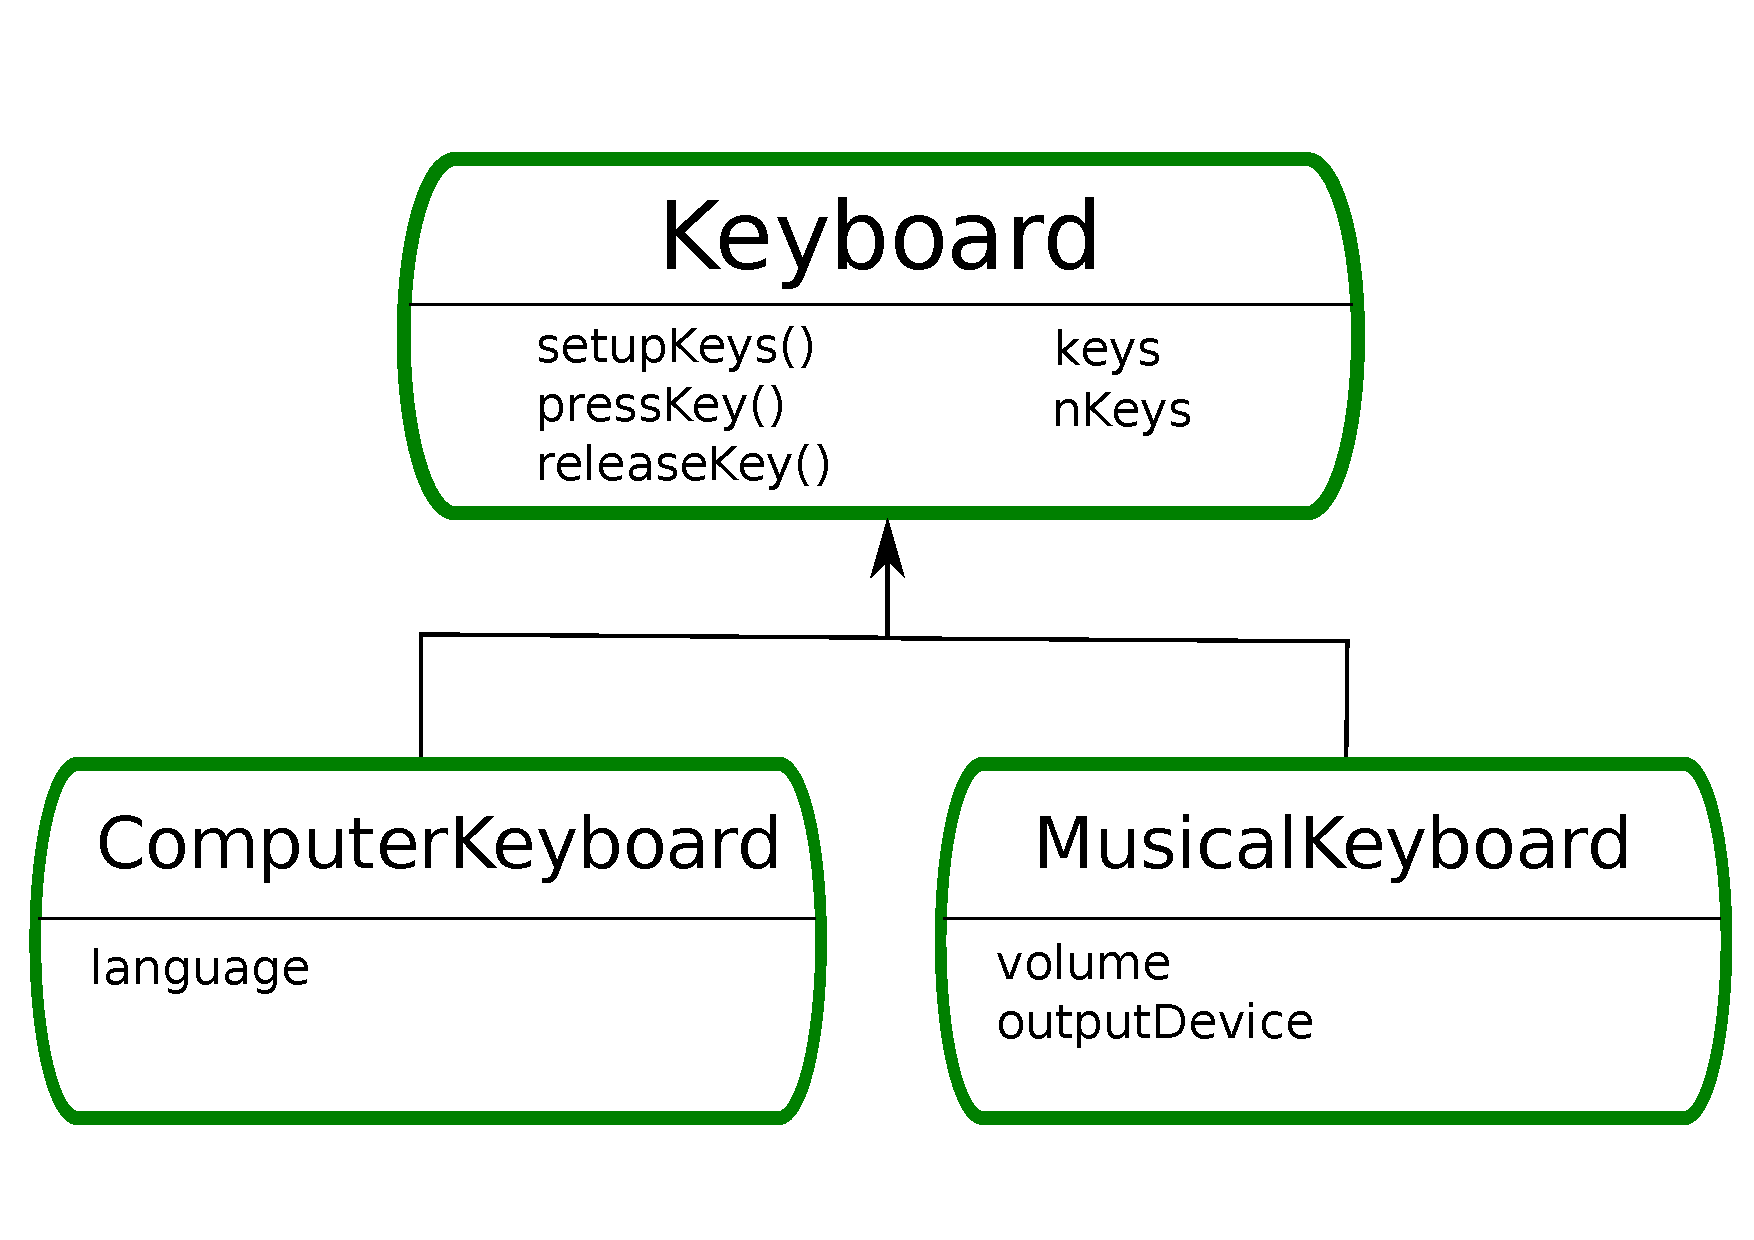
\includegraphics[scale=0.35]{../Graphics/UMLkeyboard.pdf}
  \caption{Inheritance diagram for a keyboard superclass. Class members are listed below the class name.}
  \label{fig:UMLkeyboard}
 \end{center}
\end{figure}

\clearpage
\lstinputlisting[language=Python, otherkeywords={self}]{../CodeInputs/KeyboardClassPython.py}

It is clear from looking at the superclass that two keyboards are differentiated by the way their keys are set up. Not overriding the \verb+setupKeys()+ function would cause the generic superclass constructor to call the function which would raise an exception and close the program. These kinds of superclass member functions, which requires an implementation in order for the object to be constructed, are referred to as \textit{pure virtual functions}. The other two functions do not necessarily have to be implemented, and are thus referred to as \textit{virtual} functions. These topics will be discussed in more detail in the next section.

\subsection{Pointers, Typecasting and Virtual Functions}

A pointer is a hexadecimal number representing a memory address where some \textit{type} of object is stored, for instance, an \verb+int+ at \verb+0x7fff0882306c+ (\verb+0x+ simply implies hexadecimal). Higher level languages like Python handles all the pointers and typesetting automatically. In low-level languages like C++, however, you need to control everything. This is commonly referred to as \textit{type safety}. 

Memory addresses are \textit{global}, that is, they are shared throughout the program. This implies that changes done to a pointer to an object, e.g. \verb+Keyboard* myKeyboard+, are applied everywhere the object is in use. This is particularly handy (or dangerous) when passing a pointer as an argument to a function, as changes applied to the given object will cause the object to remain changed after exiting the function. Passing non-pointer arguments would only change a local copy of the object which is destroyed upon exiting the function. The alternative would be to pass the reference to the object, e.g. \verb+&myObject+, which passes the address just as in the case of pointers. 

Creating a pointer to a keyboard object in C++ can be done in several ways. Following are three examples: 
\begin{lstlisting}
MusicalKeyboard* myKeyboard1 = new MusicalKeyboard(...);
Keyboard* myKeyboard2 = new MusicalKeyboard(...);
\end{lstlisting}

the second which is identical to 

\begin{lstlisting}
Keyboard* myKeyboard2 = (Keyboard*) myKeyboard1;
\end{lstlisting}

For reasons which will be explained in Section \ref{sec:typeCastPoly}, the second expression is extremely handy. Technically, the subclass object is \textit{type cast} to the superclass type. This is allowed since \textit{any subclass is type-compatible with a pointer to it's superclass}. Any standard functions implemented in the subclass will not be directly callable from outside the object itself, and identical functions will be overwritten by the corresponding superclass functions, unless the functions are \textit{virtual}. Flagging a function as virtual in the superclass will then tell the compiler not to overwrite this particular function when a subclass object is typecast to the superclass type.

Python does not support virtual functions in the same strict sense as C++, since typecasting is \textit{automagic} in a language which is not type safe. The following example should bring some clarity to the current topic:

\vspace{0.5 cm}
\lstinputlisting[language=c++]{../CodeInputs/virtualFunctionsC++.cpp}
\clearpage
\lstinputlisting[caption={This code demonstrates two different ways of creating an object of a subclass. In line 4, the object is created as a superclass type. Passing it to the function will cause the function to access the superclass functions unless they are declared as virtual. In line 7, the object is created as a subclass type, however, by passing it to the function, the object is typecast to the superclass type, rendering the two methods identical. In line 10, the functions are directly called, which ensures that only the subclass' functions are called regardless of them being virtual or not.}]{../CodeInputs/virtualFunctionsC++MAIN.cpp}

Executing the above code yields

\begin{verbatim}
~$ ./virtualFunctionsC++.x 
-Calling subClass object of type superClass*
subclass pure virtual override
subclass standard virtual override
superclass notVirtual

-Calling subClass object of type subClass*
subclass pure virtual override
subclass standard virtual override
superclass notVirtual

-Directly calling object of type subclass*
subclass pure virtual override
subclass standard virtual override
subclass non virtual
\end{verbatim}

As introduced in the keyboard example, the superclass in this case has a pure virtual function. Creating an object of the superclass would raise an error in the compilation, claiming that the superclass is abstract. Implemented subclasses must overload pure virtual functions in order to compile.


\subsection{Polymorphism}
\label{sec:typeCastPoly}

The previous example involved a concept referred to as \textit{polymorphism}, which is a concept closely connected to virtual functions and type casting. Because of the virtual nature of the superclass' functions, the function \verb+testFunc()+ does not a priori know its exact task. All it knows is that the received object has three functions (see the previous example). Exploiting this property is referred to as polymorphism.

Using polymorphism, codes can be written in an organized and versatile fashion. To further illustrate this, consider the following example from the Quantum Monte-Carlo (QMC) code developed in this thesis:

\clearpage
\vspace{0.5 cm}
\begin{lstlisting}[caption={An example from the QMC code. The superclass of potentials is defined by a number of particles (line 3), a dimension (line 4) and a pure virtual function for extracting the local energy of a given walker (line 10). Specific potentials are implemented as subclasses (line 14 and 24), simply overriding the pure virtual function with their own implementations.}]
class Potential {
protected:
    int n_p;
    int dim;

public:
    Potential(int n_p, int dim);

    //Pure virtual function
    virtual double get_pot_E(const Walker* walker) const = 0;

};

class Coulomb : public Potential {
public:

    Coulomb(GeneralParams &);

    //Returns the sum 1/r_i
    double get_pot_E(const Walker* walker) const;

};

class Harmonic_osc : public Potential {
protected:
    double w;

public:

    Harmonic_osc(GeneralParams &);

    //return the sum 0.5*w*r_i^2
    double get_pot_E(const Walker* walker) const;

};

...

\end{lstlisting}

Assume that an object \verb+Potential* potential+ is sent to an energy function. Since \verb+get_pot_E()+ is virtual, the potential can take any form; the energy function only checks whether it has an implementation or not. The code can easily be adapted to handle any combination of any potentials by storing the potential objects in a vector and simply accumulate the contributions:

\vspace{0.5cm}
\begin{lstlisting}
//Simple compiler definition to clean up the code
#define potvec std::vector<Potential*>

class System {

    double get_potential_energy(const Walker* walker) const;
    potvec potentials;
    ...
};

double System::get_potential_energy(const Walker* walker) const {
    double potE = 0;

    //Iterates through all loaded potentials and accumulate energies.
    for (potvec::iterator pot = potentials.begin(); pot != potentials.end(); ++pot) {
        potE += (*pot)->get_pot_E(walker);
    }

    return potE;
}
\end{lstlisting}

\subsection{Const Correctness}

In the previous \verb+Potential+ code example, function declarations with the \verb+const+ flag were used. As mentioned in the section on pointers, passing pointers to functions are dangerous business. If an object is flagged with \verb+const+ on input, e.g. \verb+void f(const x)+, the function itself cannot alter the value of \verb+x+. If it does, the compiler will abort. This property is referred to as \textit{const correctness}, and serve as a safeguard guaranteeing that nothing will happen to \verb+x+ as it passes through \verb+f+. This is practical in situations where changes to an object is unwanted.

If you declare a member function itself with \verb+const+ on the right hand side, e.g. \verb+void class::f(x) const+, no changes may be applied to class members inside this specific function. For instance, in the potential energy functions, all that is requested is to evaluate a function at a given set of coordinates; there is no need to change anything, hence the const correctness is applied to the function. 

In other words: const correctness works as a safeguard preventing changes to values which should remain unchanged. A change in such a variable is then followed by a compiler error instead of unforeseen consequences.

\subsection{Accessibility levels and Friend classes}

When a C++ class is declared, each member needs to be related to an \textit{accessibility level}. The three accessibility levels in C++ are 

\begin{enumerate}[label=\textbf{(\roman{*})}, ref=(\roman{*}), align=left]
 \item \textbf{Public:}\qquad The variable or function may be accessed from anywhere the object is available.
 \item \textbf{Private:}\quad\, The variable or function may be accessed only from within the class itself. 
 \item \textbf{Protected:} As for private, but also accessible from subclasses of the class.
 \label{enum:accessibilityLevels}
 \vspace{0.3cm}
\end{enumerate}

As an example, any standardized application (app) needs the \verb+app::execute_app()+ function to be public, i.e.~accessible from the main file. On the other hand, \verb+app::dump_progress()+ should be controlled by the application itself, and should thus be private, or protected in case the application has subclasses.

There is one exception to the rule of protected - and private variables. In certain situations where a class needs to access private variables from another class, but going full public is undesired, the latter class can \textit{friend} the first class. This implies that the first class has access to the second class' private members.

In the QMC code developed in this thesis, the distribution is calculated by a class \verb+Distrubution+. In order to achieve this, the protected members of \verb+QMC+ need to be made available to the \verb+Distrubution+ class. This is implemented in the following fashion:

\clearpage
\begin{lstlisting}[language=c++, caption={An example from the QMC code. The distribution class needs access to the private members of QMC. This is achieved in line 13 by friending the distribution class.}]

class QMC {
protected:
    
    arma::mat dist; //!< Matrix holding positional data for the distribution.
    int last_inserted; //!< Index of last inserted positional data.
    ...

public:
    ...

    //Gives Distribution access to protected members of QMC.
    friend class Distribution;

};

void Distribution::finalize() {

    //scrap out all the over-allocated space (DMC)
    qmc->dist.resize(qmc->last_inserted, dim);

    if (dim == 3) {
        generate_distribution3D(qmc->dist, qmc->n_p);
    } else {
        generate_distribution2D(qmc->dist, qmc->n_p);
    }

    qmc->dist.reset();

}
\end{lstlisting}

Codes could be developed without using \verb+const+ flags and with solely public members, however, in that case it is very easy to put together a very disorganized code, with pointers going everywhere and functions being called in all sorts of contexts. This is especially true if there are several developers on the same project. 

Clever use of accessibility levels will make codes easier to develop in an organized and intuitive fashion Put in other words: If you have to break an accessibility level to implement a desired functionality, there probably exists a better way of implementing it.


\subsection{Example: PotionGame}
\label{sec:PotionGame}

To conclude this section on object orientation, consider the following code for a player vs. player game:
\clearpage

\vspace{0.5 cm}
\lstinputlisting[language=Python, otherkeywords={self}]{../CodeInputs/playerClass.py}
\clearpage
\lstinputlisting[language=Python, otherkeywords={self}]{../CodeInputs/potionClass.py}

The \verb+Player+ class keeps track of everything a player needs of personal data, such as the name (line 10), health- and  energy levels (line 8), potions etc. Bringing another player into the game is simply done by creating another \verb+Player+ object. A player holds a number of \verb+Potion+ objects in a list (line 14). These objects are subclass implementations of the abstract potion class, which overwrites the virtual function describing the potion's effect on a given player object. This is demonstrated in lines 23 and 32. This subclass hierarchy of potions makes it incredibly easy to implement new ones.

The power of object orientation shines through in this simple example. The readability is very good, and does not falter if numerous potions or players are brought to the table.

In this section the focus has not been solely on scientific computing, but rather on the use of object orientation in general. The interplay between the potions and the players in the current example closely resembles the interplay between the QMC solver and the potentials introduced previously. Whether games or scientific programs are at hand, the methods used in the programming remain the same. 

On the following page, a game is constructed using the \verb+Player+ and \verb+Potion+ classes. In lines 15-22, three players are initialized with a set of potions, from where they battle each other one round. The syntax is extremely transparent. Adding a fourth player is simply a matter of adding a new line of code. The output of the game is displayed below the code. 
 
\clearpage
\lstinputlisting[language=Python, otherkeywords={self}]{../CodeInputs/potionGameMain.py}

\scriptsize
\begin{verbatim}
Round start: 
  Sigve (hp/e=100/100):
  Energy Potion (10)

  Jorgen (hp/e=100/100):
  Health Potion (20)
  Energy Potion (20)

  Karl (hp/e=100/100):
  Health Potion (20)

Sigve hit Jorgen for 40 using 55 energy
Sigve: Insuficcient energy to attack.
Sigve consumes Energy Potion (10).
Sigve hit Karl for 35 using 55 energy

Karl consumes Health Potion (20).
Karl hit Sigve for 41 using 55 energy

Jorgen hit Karl for 44 using 55 energy
Jorgen consumes Energy Potion (20).
Jorgen hit Sigve for 47 using 55 energy

Round 1: 
  Sigve (hp/e=12/0):
  No potions available

  Jorgen (hp/e=60/10):
  Health Potion (20)

  Karl (hp/e=41/45):
  No potions available
\end{verbatim}
\clearpage
\normalsize

\section{Structuring the code}

Structuring a code is a matter of making choices based on the complexity of the code. If the code is short and has a direct purpose, for instance, to calculate the sum from Eq.~(\ref{eq:sum100}), the structure is not an issue at all, given that reasonable variable names are used. However, if the code is more complex and the methods used are specific implementations of a more general case, e.g.~potentials, code structuring becomes very important. For details about the structuring of the code used in this thesis, see the documentation provided in Ref. \cite{libBorealisCode}. 

\subsection{File Structures}

Not only does the potion game example demonstrate clean object orientation, but also standard file structuring by splitting the different classes and the main application into separate files. In a small code, like for example the potion game, the gain of transparency is not immense, however, when the class structures span thousands of lines, having a good structure is crucial to the development process, the code's readability, and the management in general.

Developing codes in scientific scenarios often involve large frameworks. For example, when coding molecular dynamics, several collision models, force models etc. are implemented alongside the main solver. In the case of Markow Chain Monte Carlo methods, different diffusion models (sampling rules) may be selectable. Even though these models are implemented using polymorphism, the code still gets messy when the amount of classes  gets large. 

In these scenarios, it is common to gather the implementations of the different classes in separate files (as for the potion game). This would be for purely cosmetic reasons if the process of writing code was linear, however, empirical evidence suggests otherwise: At least half the time is spent debugging, going back and forth between files. 

A standard way to organize code is to have all the source code gathered in a \textit{src} folder, with one folder per distinct class. Subclasses should appear as folders inside the superclass folder. Figure \ref{FIG:SRCdirTree} shows an example setup for the framework of an object oriented code.



Another gain by this structuring files this way, is that tools such as Make, QMake, etc. ensures that only the files that actually changed will be recompiled. This saves a lot of time in the development process once the total compilation time starts taking several minutes.

\subsection{Class Structures}

In scientific programming, the simulated process often has a physical or mathematical interpretation. Some examples are, for instance, atoms in molecular dynamics and Bose-Einstein condensates, random walkers in diffusion processes, etc. Implementing classes representing these quantities will shorten the gap between the mathematical formulation of the problem and the implementation.

In addition, quantities such as the energy, entropy and temperature, are all calculated based on equations from statistical mechanics, quantum mechanics, or similar. Having class methods representing these calculations will again shorten the gap. There is no question what is done when the \verb+system.get_potential_energy+ method is called, however, if some random loop appears in the main solver, an initial investigation is required in order to understand the flow of the code.

As described in Section \ref{sec:typeCastPoly}, abstracting for example the potential energy function into a system object opens up the possibility of generalizing the code to any potential without altering the main solver. Structure is in other words vital if readability and versatility is desired. 

Planning the code structure comes in as a key part of any large coding project. For details regarding the planning of the code in this thesis, see Section \ref{sec:AssGoal}.

\begin{figure}[h]
 
 \begin{center}
  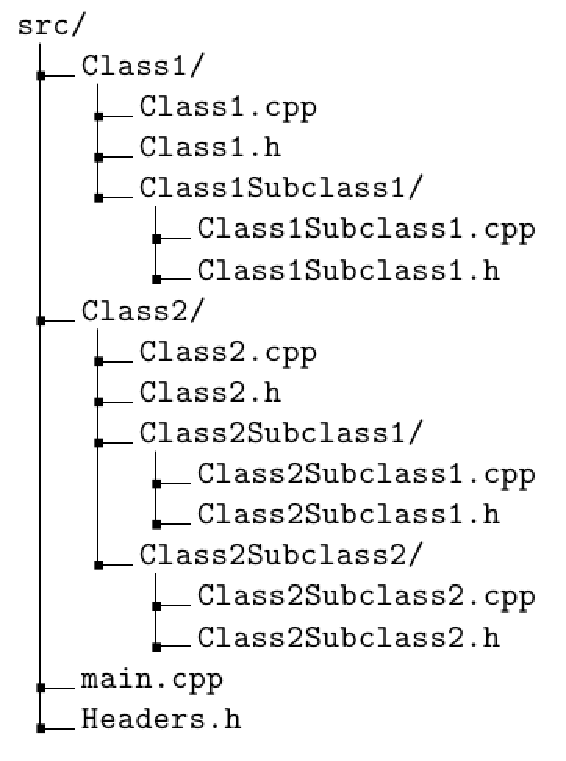
\includegraphics[scale=0.6]{../Graphics/SRCfolderStruct.pdf} 
 \end{center}

 \caption{An illustration of a standard way to organize source code. The file endings represent C++ code.}
 \label{FIG:SRCdirTree}
\end{figure}
